\documentclass{article}

%%%%%%%%%%%%%%%%%%%%%%%%%%%%%%%%%%%%%%%%

\usepackage[utf8]{inputenc}

%%%%%%%%%%%%%%%%%%%%%%%%%%%%%%%%%%%%%%%%

\usepackage{tikz}
\usepackage{pgfplots}
\pgfplotsset{compat=1.13}

%%%%%%%%%%%%%%%%%%%%%%%%%%%%%%%%%%%%%%%%

\usepackage{amsmath,amsfonts,amssymb}
\renewcommand{\baselinestretch}{1.0}
\usepackage{graphicx}
\usepackage[colorlinks=true, allcolors=blue]{hyperref}
\usepackage{lscape}

%%%%%%%%%%%%%%%%%%%%%%%%%%%%%%%%%%%%%%%%

\setlength{\parindent}{0pt}
\setlength{\parskip}{\medskipamount}

%%%%%%%%%%%%%%%%%%%%%%%%%%%%%%%%%%%%%%%%

\usepackage{newtxtext,newtxmath}

% Instead of the above, use this for arXiv:

%\usepackage{txfonts}
%\usepackage{textcomp}
%\usepackage{eurosym}
%\let\texteuro\euro

%%%%%%%%%%%%%%%%%%%%%%%%%%%%%%%%%%%%%%%%

\newcommand{\unit}[1]{\ensuremath{\mathrm{#1}}}
\newcommand{\micron}{\mbox{$\mu$m}}
\renewcommand{\deg}{\mbox{deg}}
\newcommand{\sqdeg}{\mbox{$\deg^2$}}
\newcommand{\persqdeg}{\mbox{$\deg^{-2}$}}
\newcommand{\arcmin}{\mbox{arcmin}}
\newcommand{\sqarcmin}{\mbox{\arcmin$^2$}}
\newcommand{\persqarcmin}{\mbox{\arcmin$^{-2}$}}
\newcommand{\arcsec}{\mbox{arcsec}}
\newcommand{\sqarcsec}{\mbox{\arcsec$^2$}}
\newcommand{\persqarcsec}{\mbox{\arcsec$^{-2}$}}
\newcommand{\sqmm}{\mbox{mm$^2$}}
\newcommand{\deighty}{\ensuremath{d_{80}}}

\newcommand{\variable}[1]{\ensuremath{\left<\mathit{#1}\right>}}

%%%%%%%%%%%%%%%%%%%%%%%%%%%%%%%%%%%%%%%%

\newcounter{requirement}

\newcommand{\requirement}[3]{
 \stepcounter{requirement}
 \subsection*{VIS-\therequirement: #1}
 {\bfseries Requirement: }#2\par
 {\bfseries Source: }#3\par
}

\newcommand{\comment}[1]{\begin{quotation}\noindent\itshape #1\end{quotation}}

%%%%%%%%%%%%%%%%%%%%%%%%%%%%%%%%%%%%%%%%

\begin{document}

\pagestyle{empty}

\pagestyle{empty}

\begin{center}
\Large \bfseries 
DDRAGO and WOB\\
Control System Design
\end{center}

\begin{center}
\begin{tabular}{ll}
Prepared by:&Fernando Angeles\\
&Alan M. Watson\\
Revised by:&Alan M. Watson\\
& Rosalía Langarica\\
Approved by:&Alan M. Watson\\
& Rosalía Langarica\\
Reference:&COLIBRI-UNAM-DS-7\\
Version:&1.5\\
Date:&16 February 2022\\
\end{tabular}
\end{center}

\vspace{\fill}

\begin{center}
DDRAGO Project\\
Instituto de Astronomía\\
Universidad Nacional Autónoma de México
\end{center}

\newpage
\section*{Document Change Record}

\begin{itemize}

\item Version 1.6 of 12 February 2024.
\begin{itemize}
    \item The fibers for the USB extender are OM2, not OM1.
\end{itemize}

\item Version 1.5 of 16 February 2022.
\begin{itemize}
    \item Backup power will now be provided by the building UPS.
\end{itemize}


\item Version 1.4 of 29 March 2022.
\begin{itemize}
    \item Explicitly specified in \S2.1 that the detector format and that they have shutters, as required by the FPRD.
    \item Removed computers that are really part of the telescope control system.
    \item Noted that all cables will be labelled.
\end{itemize}

\item Version 1.3 of 15 March 2022.
\begin{itemize}
    \item Correction of the total power budget in \S4.2
\end{itemize}

\item Version 1.2 of 23 February 2022.
\begin{itemize}
    \item Added characteristics of the linear stage and shutter.
    \item Corrected nomenclature.
    \item Corrected cabling and hoses diagram.
    \item Corrected Cables and Hoses Between the Control Room and Instrument.
    \item Corrected cables and fibers through the azimuth cable wrap table.
    \item Corrected section Cables, Hoses, and Fibers.
    \item Corrected inconsistencies between radius and diameters for the cables.
    \item Added a comment on the lack of an installed spare main power cable.
    \item Added a comment on the need to fill the evacuated spare hoses before they are used.
\end{itemize}

\item Version 1.1 of 2 February 2022.
\begin{itemize}
    \item Added descriptions of the shutter and linear stage.
    \item Added the USB hub.
\end{itemize}

\item Version 1.0 of 30 January 2022.
\begin{itemize}
    \item Initial version modified from version 2.2 of the corresponding DDRAGUITO document.
\end{itemize}

\end{itemize}


\newpage

\pagestyle{plain}

\tableofcontents

\clearpage
\section{Architecture}

The control system hardware is physically located in two areas: on the instrument and in the control room. The hardware is connected by cables and hoses that run from the control room through the building, the telescope, the azimuth and elevation cable wraps, and to the instrument. The architecture is shown in Figure~\ref{figure:electronics-architecture}.

\begin{figure}[bp]
\begin{center}
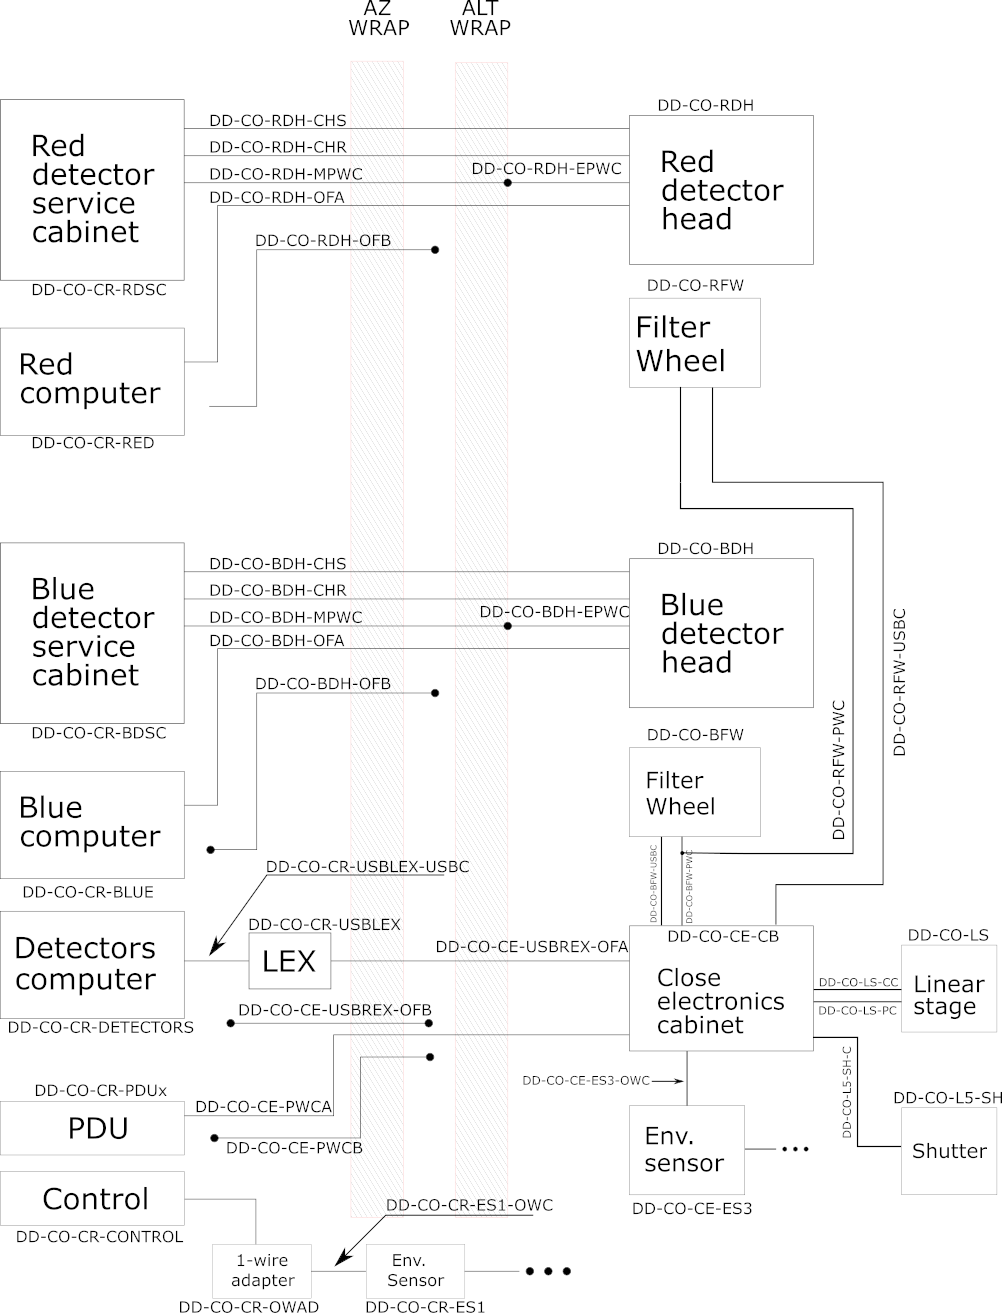
\includegraphics[width=0.9\linewidth]{figures/electronics-architecture.png}
\end{center}
\caption{The control system architecture.}
\label{figure:electronics-architecture}
\end{figure}


\clearpage
\section{Hardware on the Instrument}

\subsection{Detectors}
\label{section:detectors}

The DDRAGO instrument uses two Spectral Instruments 1110S CCD detector systems with a backside-illuminated e2v 2331-84 CCD (DD-CO-BDH and DD-CO-RDH). These detectors have a format of $4\mathrm{k}\times4\mathrm{k}$ with 15~{\micron} pixels. The blue detector works in $gri$ and the red detector in $zy$. The detectors have the “astro multi-2” AR coating and deep-depleted silicon. The red detector also has e2v's fringing-suppression treatment. They are cooled by a Brookes Polycold® PCC Compact Cooler with PT-30 refrigerant. Each detector has an integrated Vincent/Uniblitz CS90HS1T0 shutter. These detectors are referred to as the “blue detector" and "red detector”.

The properties of the detectors are described in more detail in the document “COLIBRÍ Expected Performance”.

The CCDs are controlled by two Windows computers (DD-CO-CR-BLUE and DD-CO-CR-RED) in the control room over fibre optic link, they are powered by a custom power supply and supplied with pressurized PT-30 gas from two compressors, both housed in a vendor-supplied service cabinet (DD-CO-CR-BDSC and DD-CO-CR-RDSC) in the control room.

There are four OM1 MT-RJ two-strand optical fibers from the computer in the control room to the blue and red detector head, two in-service (DD-CO-BDH-OFA and DD-CO-RDH-OFA) and one spare (DD-CO-BDH-OFB and DD-CO-RDH-OFB). There are two two-part power cables (DD-CO-BDH-MPWC - DD-CO-BDH-EPWC and DD-CO-RDH-MPWC - DD-CO-RDH-EPWC) and four cryogen hoses, one supply and one return for each (DD-CO-BDH-CHS, DD-CO-BDH-CHR, DD-CO-RDH-CHS, and DD-CO-RDH-CHR) from the service cabinet in the control room to the blue detector head. 

A spare pair of evacuated hoses run from the control room to the azimuth base. These can be used either by DDRAGO or CAGIRE. They are evacuated, since DDRAGO and CAGIRE use different refrigerant gases.

We will have a spare cylinder of PT-30 gas and a filling hose on-site to enable us to maintain the pressure after minor leaks (e.g., from connecting and disconnecting the cables) and to fill the spare hoses.

\subsection{Filter Wheels}

DDRAGO uses two FLI CFW14-5 filter wheels (DD-CO-BFW and DD-CO-RFW). This is a custom adaptation by FLI for five 76 mm square filters.

The filter wheels are controlled by USB via a USB extender (DD-CO-CR-USBLEX and DD-CO-CE-USBREX) from the TCS detectors computer (DD-CO-CR-DETECTORS).

The filter wheels require 12 VDC 15 W (1.25 A each one) and is supplied from a power supply in the close electronics cabinet (DD-CO-CE-PS12). Assuming a 10\% duty cycle, the mean power is 3 W.

We will have a spare filter wheel on site.

\subsection{Environmental Sensors}

We use 1-wire sensors for environmental monitoring. These connect in series to a LinkHUBi masters (DD-CO-CE-OWAD) which are on the USB buses to the TCS detectors computer (DD-CO-CR-DETECTORS). The USB connection from DD-CO-CR-DETECTORS to DD-CO-CE-OWAD in the the close electronics is via the USB extender (DD-CO-CR-USBLEX and DD-CO-CE-USBREX).

The 1-wire connections use standard Cat~5 UTP cable and RJ45 connectors. Note that although Cat~5 UTP cable and RJ45 connectors are also used for Ethernet connections, the 1-Wire protocol is not compatible with Ethernet. To distinguish the two in other projects at the OAN, we use yellow for 1-Wire cables and other colors for Ethernet cables. We use this convention in DDRAGO.

We use iButtonLink MS-T and MS-TH 1-Wire temperature and humidity sensors for environmental monitoring (DD-CO-CE-ES2/3/4/5/6/7/8). The MS-T sensor measures temperature over an operating range of $-40$ C to $+85$ C and has a precision typically of $\pm 2$ C. The MS-TH measures temperature like the MS-T and also humidity. The MS-TH sensor has an operating range 0\% to 100\% relative humidity and has a precision typically of $\pm 3.5\%$ relative humidity, which is adequate for our purposes. We have calibrated the temperature offsets of the sensors and spares to a fiducial sensor at least two temperatures, in order to improve the differential sensitivity to better than 1~C.

The iButtonLink line does not have a pressure sensor. Therefore, to measure pressure we use an EDS OW-ENV-THPL 1-wire sensor (DD-CO-CE-ES1), mounted on the outside of the electronics box. This also measures temperature, humidity, and light level.

The following sensors are connected to the bus in the close electronics cabinet:
\begin{itemize}
\item One OW-ENV-THPL-1 outside the close electronics cabinet (DD-CO-CE-ES1).
\item One MS-TH inside the close electronics cabinet (DD-CO-CE-ES2)
\item Three MS-TH inside the instrument at the position shown in the mechanical design document (DD-CO-CE-ES3/4/5).
\item Three MS-TH outside the instrument exposed to the derotator tunnel (DD-CO-CE-ES6/7/8). Only one is connected, but others are hot spares and can be selected by simply changing the cable that connects them to DD-CO-CE-ES5. We have chose this approach since access to the tunnel requires removing the instrument.
\end{itemize}

\subsection{Close Electronics Cabinet}

The instrument close electronics cabinet (DD-CO-CE-CB) is physically mounted on the instrument. The cabinet provides a temperature-controlled environment for the power supplies and the electronics that provide USB and 1-Wire buses on the instrument.

\begin{figure}[tp]
\begin{center}
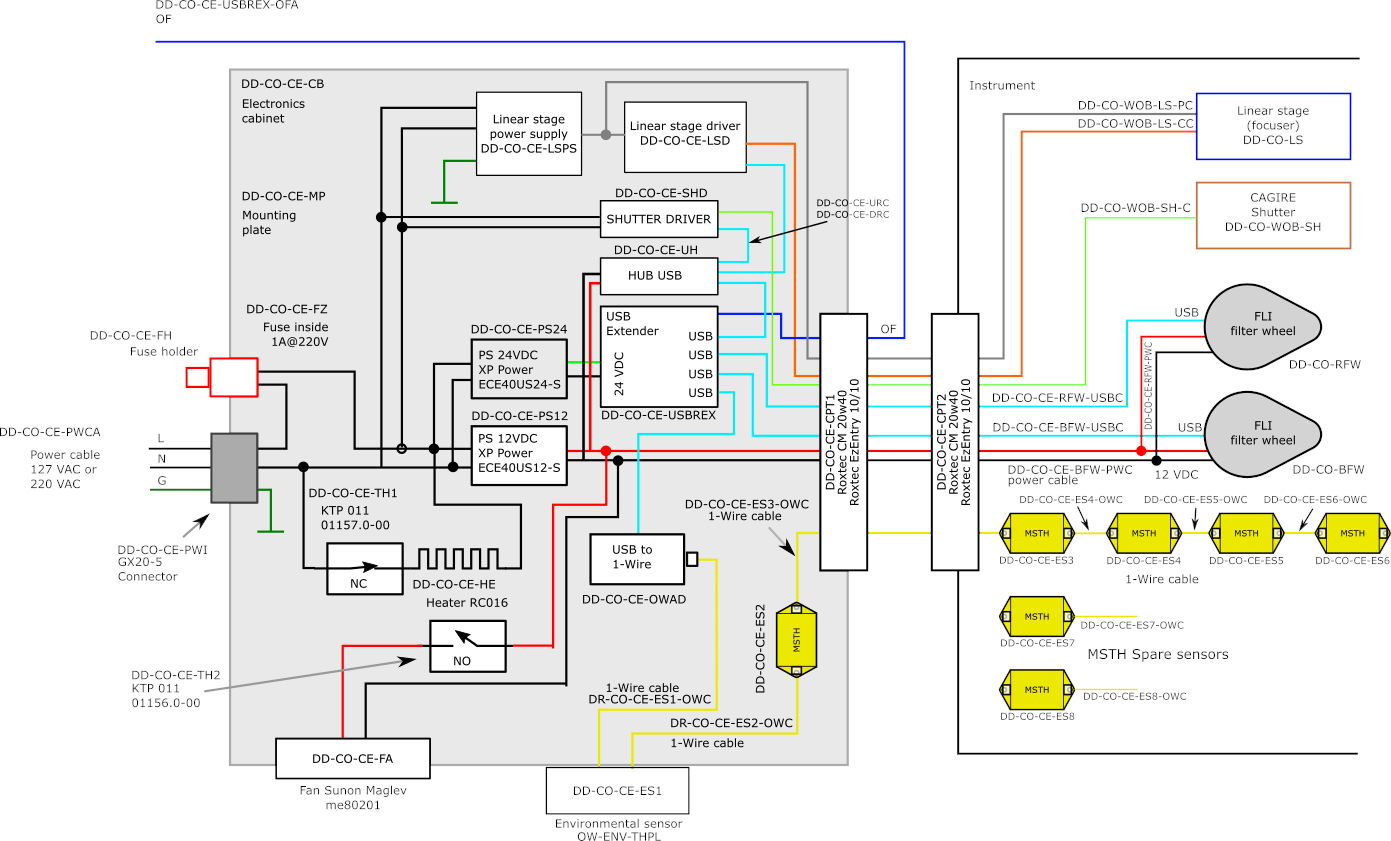
\includegraphics[height=0.9\linewidth,angle=90]{figures/CloseElectronics}
\end{center}
\caption{Schematic Diagram of the Close Electronics (DD-CO-CE).}
\label{figure:electronics-cabinet}
\end{figure}

%\begin{figure}[tp]
%\begin{center}
%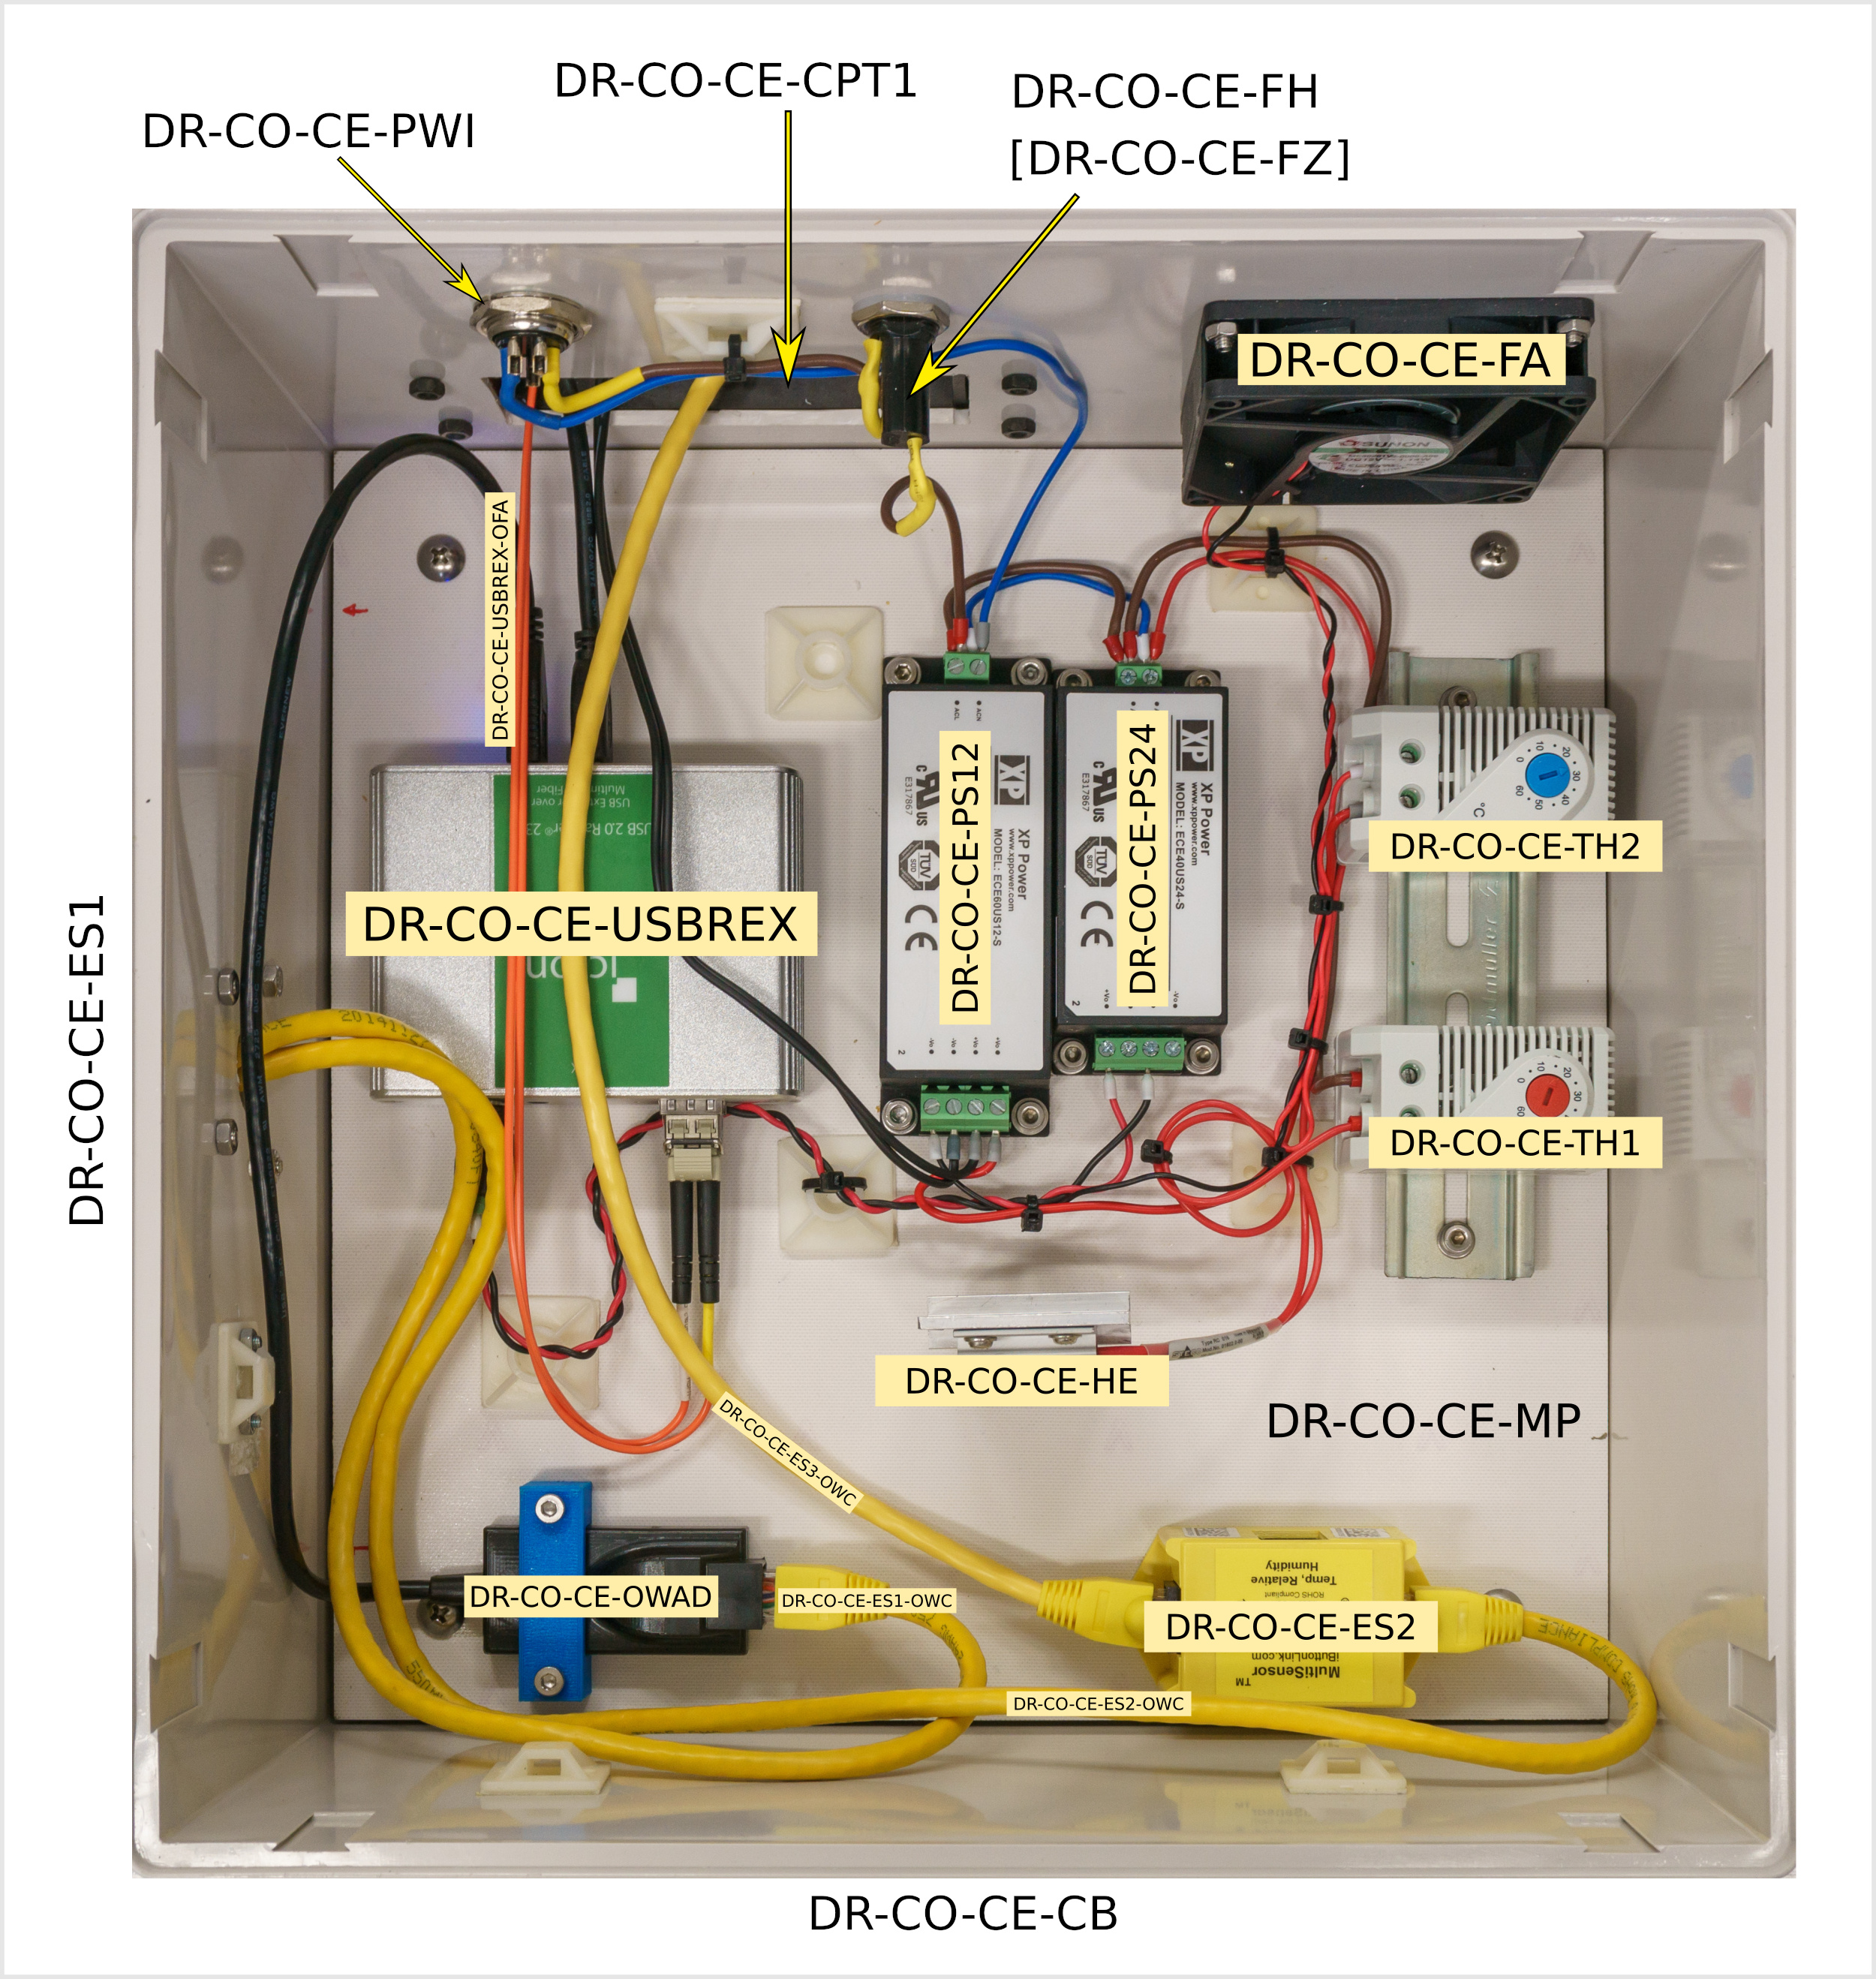
\includegraphics[width=0.9\linewidth]{figures/electronics-cabinet-photo.jpg}
%\end{center}
%\caption{A Photo of the Close Electronics Cabinet (DD-CO-CE).}
%\label{figure:electronics-cabinet-photo}
%\end{figure}

A schematic diagram of the electronics cabinet is shown in Figure~\ref{figure:electronics-cabinet}. 
%A photo is shown in Figure~\ref{figure:electronics-cabinet-photo}

All cables to and from the electronics cabinet use appropriate connectors or cable seals with appropriate strain relief.

\subsubsection{Cabinet}

The cabinet itself (DD-CO-CE-CB) is a Bud Industries NBB-15245. This cabinet is moulded in ABS and is approximately $330 \times 330 \times 180$ mm. The advantage of this relatively large cabinet is that it gives good access to all of the installed components. The components within the cabinet are mounted on a mounting plate (DD-CO-CE-MP), which can be removed to facilitate maintenance.

\subsubsection{Mains Supply}

\begin{figure}[tp]
\begin{center}
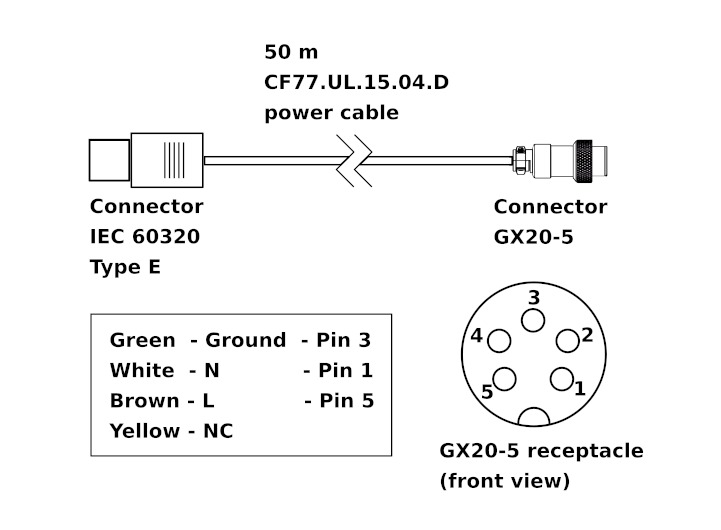
\includegraphics[width=0.9\linewidth]{figures/DR-CO-CE-PWC}
\end{center}
\caption{Wiring diagram for the cables DD-CO-CE-PWCA/B.}
\label{figure:DD-CO-CE-PWC}
\end{figure}

There are two mains supply cables from an iBoot PDU in the control room, one in-service (DD-CO-CE-PWCA) and one spare (DD-CO-CE-PWCB).

Both cables terminate in MIL GX20-5 plugs, with pin 1 being neutral, pin 3 being ground, and pin 5 being live. This is shown in Figure~\ref{figure:DD-CO-CE-PWC}
There is a MIL GX20-5 socket on the instrument electronics cabinet. None of our equipment requires earthing, so although we run earth to the cabinet it is not be connected beyond the connector.

The mains supply have an externally-accessible 1~A fuse (DD-CO-CE-FZ in the holder DD-CO-CE-FH).

All of the components in the electronics cabinet are compatible with both 127 V 60 Hz and 230 V 50 Hz.

\subsubsection{Thermal Control System}

The thermal control system consists of a thermostat-controlled heater and a thermostat-controlled fan. We use a Stego KT 01157.0-00 NC thermostat for the heater (DD-CO-CE-TH1) and a Stego KT 01156.0-00 NO thermostat for the fan (DD-CO-CE-TH1), a Stego RC 01602.0-00 heater (DD-CO-CE-HE), and Sunon Maglev me80201 V2-0000-A99 low-vibration fan (DD-CO-CE-FA). 

The heater requires 127/220~VAC 8~W and the fan 12~VDC 1~W. The thermostats are compatible with 12 VDC and 127/220 VAC. The fan is supplied by the 12 VDC power supply (DD-CO-CE-PS12). The heater is supplied directly from the general 127/220 VAC supply to the cabinet.

All of the components of the thermal control system are rated to operate over the entire \emph{survival} range of the instrument ($-25$ to $+35$~C): the thermostats from $-45$ to $+80$~C, the heater from $-45$ to $+70$~C, and the fans from $-30$ to $+60$ C. As such, we do not expect to have to shut down the thermal control system except for maintenance or during power failures.

%The thermostats and heater are rated for operation at both 127 V 60 Hz and 230 V 50 Hz. The fans are not; we will use the 127 V 60 Hz model 109-042UL in the OAN and the 230 V 50 Hz 109-044UL model in the OHP. These two models are mechanically identical.

The thermostats can be adjusted to switch between $-15$~C and $+45$~C. They are set to turn the heater on below $-10$~C and turn the fans on above $-5$~C. Thus, the temperature in the enclosure could potentially fall to $-10$~C, which is formally outside the range of the digital equipment installed in the cabinet. Nevertheless, we have successfully operated nearly identical digital equipment in the dome of the 1.5-meter telescope for ten years at temperatures reaching $-11$~C. Therefore, we anticipate that maintaining the temperature above $-10$~C will be perfectly adequate. If for some reason, we do have problems at $-10$~C, we will adjust the thermostats to maintain the electronics at a higher temperature.

The heat from cabinet is exhausted directly into the dome. However, we expect it to be about 9 W (1 W for the power supplies, 1 W from the fans, 7 W for the USB extender). Furthermore, except below $-5$ C, we expect this heat will be heavily diluted into the flow of ambient-temperature air driven by the fans.

\subsubsection{Power Supplies}

The filter wheels and fan require 12 VDC power and the USB extender and the shutter require 24 VDC power. We propose use an XP Power ECE40US12-S (DD-CO-CE-PS12) which supplies 12~VDC 40~W and an XP Power ECE40US24-S (DD-CO-CE-PS24) which supplies 24~VDC 40~W. These accept 85--264 VAC 47--63 Hz. They have an operating temperature range of $-25$ to $+70$ C.

The linear stage requires 24~VDC 2.1~A for the motor and the controller. The power supply is proprietary and is connected to AC. The operation time is reduced and intermittent.

The shutter driver includes its own power supply and is connected to AC.

We expect the average/maximum loads to be about 2.5/16 W on the 12 V power supply, 1/24 W on the 24 V power supply and 2/5 W on the linear stage in total. Assuming an 80\% efficiency, the average dissipation is about 5 W in total.

All of the power supplies are compatible with both 120 V 60 Hz and 240 V 50 Hz.

\subsubsection{USB Extender}

The cabinet contains a Icron Ranger 2324 USB 2.0 extender. The remote unit (DD-CO-CE-USBREX) is in the close electronics cabinet and the local unit (DD-CO-R-USBLEX) is in the control room and connected to the USB bus from the TCS detectors computer (DD-CO-CR-DETECTORS). 

The local and remote units are connected by an OM2 two-strand fibers with LC connectors. There are two cables, one in-service (DD-CO-CE-USBREX-OFA) and one spare (DD-CO-CE-USBREX-OFB).

%The extender has four USB ports, and we use two for the filter wheels (DD-CO-BFW and DD-CO-RFW), one for the 1-wire adapter (DD-CO-CE-OWAD) and one for the linear stage.

The extender formally requires 24~VDC 24~W (1~A), but 20~W of this is to supply 5~W of power to each USB port. Since the USB bus will control only digital devices, we expect the actual total power to be 10~W or less.

The thermal control system maintains the electronics cabinet above $-10$~C. The operating temperature range of the extender is given as 0 to 50~C, but as we noted above we have operated similar extenders at the 1.5 meter telescope for ten years at temperatures as cold as $-11$~C without problems. We prefer not to heat the cabinet to avoid turbulence inside the dome and heat dissipation in excess.

\subsubsection{USB HUB}
Five USB ´ports are needed to control all of the components inside the cabinet, we include a 4-port USB hub Startech ST4200USBM (DD-CO-CE-UH) to increase the number of the four available USB ports from (DD-CO-CE-USBREX). 

This hub is powered by the 12 VDC power supply and includes a USB cable to the USB extender (DD-CO-CE-HC). The VCM-D1 Shutter Driver DD-CO-CE-SHD and the controller of the linear stage DD-CO-WOB-LS-D are attached to this hub.

\subsubsection{Shutter}
The shutter for Cagire DD-CO-LS-SH is an  un-housed 6 blades Uniblitz CS90HS1T0 with an aperture of 90 mm.It is driven with its own VCM-D1 Shutter Driver (DD-CO-CE-SHD). Its opening time is 66 ms and is specifically designed to suit astronomical applications. The operating temperature is 0 C to 80 C and weighs 320 g.

\subsubsection{Shutter driver}
The shutter for Cagire is controlled with a Uniblitz VCM-D1 Shutter Driver located inside the cabinet (DD-CO-CE-SHD). 

This driver is powered with 120 VAC @ 60W. Commands are sent from the control computer via a USB to RS232 adapter Manhattan Part No. 205153 (DD-CO-CE-URC) connected to the USB extender (DD-CO-CE-USBREX) and an assembled cable that converts DB9 to RJ45 (DD-CO-CE-DRC).

\subsubsection{Linear stage}
The linear stage DD-CO-WOB-LS works as a focuser on the WOB. This is a Physik Instrumente M-126.PD1 Microtranslation stage with a travel range of 25 mm  with a maximum speed of 50 mm/s, repeatability is 0.1 µm and minimum incremental motion 0.1 µm. Its operating temperature range is -20 C to 65 C. It is controlled from DD-CO-WOB-LS-D connected with a proprietary cable DD-CO-WOB-LS-CC with DB15 connectors and receives power from DD-CO-WOB-LS-PS through the modified cable DD-CO-WOB-LS-PC. The power supply DD-CO-WOB-LS-PS only has one output. Therefore we will modify the commercial cable DD-CO-WOB-LS-PC so that the power supply can power both the linear stage and the linear stage driver.
Two linear stages were acquired, one for installation and one for spare. 

\subsubsection{Linear stage driver}
The linear stage is controlled with a proprietary driver Mercury servo controller C863.12 (DD-CO-WOB-LS-D) located inside the cabinet. This driver is controlled via USB from DD-CO-CE-UH. It is powered by the power supply DD-CO-WOB-LS-PS located inside the cabinet which also powers the linear stage.


\subsubsection{1-Wire Adapter}

The cabinet also contains an iButtonLink LinkUSBi 1-Wire USB adapter (DD-CO-CE-OWAD). This is a 1-Wire master with a USB interface. It is powered by the USB bus. It provides the detectors computer in the control room with a 1-Wire bus on the instrument.

The thermal control system maintains the electronics cabinet at $-10$~C or above. The operating temperature range of the adapter is not listed by the vendor. However, we have operated similar LinkUSB-E devices at the 1.5 meter telescope for eleven winters at temperatures as cold as $-11$ C without problems and identical LinkUSBi adapters at the COATLI telescopes for five winters without problem. 

\subsubsection{Cable Seals}

Seven cables go from the instrument electronics cabinet into the instrument itself: one 12 VDC power cable for the filter wheels (DD-CO-BFW-PWC), two USB cable for the filter wheels (DD-CO-BFW-USBC and DD-CO-RFW-USBC), one Cat-5 UTP cable for the 1-wire sensors (DD-CE-ES3-OWC), one proprietary cable for the control of the linear stage (DD-CO-CE-LSC), one cable to operate the shutter (DD-CO-L5-SH-C) and one cable for the linear stage motor (DD-CO-CE-LSPC).

The cables leave the electronics cabinet through a cable pass-through (DD-CO-CE-CPT1) consisting of a Roxtec EzEntry 10 frame with Roxtec CM 20w40 inserts mounted over a slot in the cabinet wall. They enter the instrument using a similar cable pass-thru (DD-CO-CE-CPT2) in the instrument support structure. Each cable pass-through is capable of passing 10 cables from 3.5 to 16.5 mm in diameter. 

The cables to and from the OW-ENV-THPL sensor mounted on the electronics box enter and leave the sensor from behind. Therefore, we have simply drilled a suitable hole in the cabinet behind the sensor for these cables.

\subsubsection{Fibers}

Communication with the USB extender is over a OM2 two-strand fibers with LC connectors. The fibre enters through the Roxtec CM 20w40 cable pass-thru (DD-CO-CE-CPT1)  mounted on the electronics box.

\clearpage
\section{Hardware in the Control Room}

\subsection{19-inch Rack}

The hardware in the control room is largely mounted in a standard 19-inch rack. Note that the hardware here includes the computers to run the TCS. The hardware includes:

\begin{itemize}
\item
Two 24-port 1000BASE-TX Ethernet switches (DD-CO-CR-SWITCH with a spare DD-CO-CR-SPARESWITCH). This provides a LAN for the computers and the iBootBars PDUs.
%\item
%One Mac mini access computer called “access” (DD-CO-CR-ACCESS with a spare DD-CO-CR-SPAREACCESS) on a 1U shelf.
\item
One CCD computer called “blue” (DD-CO-CR-BLUE). This runs Windows 10. It is equipped with a custom PCIe card from Spectral Instruments (DD-CO-CR-BLUE-DPC) to control the blue CCD via an optical fiber and runs the Spectral Instruments Windows control software.
\item
One CCD computer called “red” (DD-CO-CR-RED). This runs Windows 10. It is equipped with a custom PCIe card from Spectral Instruments (DD-CO-CR-RED-DPC) to control the red CCD via an optical fiber and runs the Spectral Instruments Windows control software.
\item
One detectors computer called “detectors” (DD-CO-CR-DETECTORS). This runs Linux Ubuntu 18.04 LTS server. It will control the CCD (via the Spectral Instruments TCP/IP interface on blue) and the filter wheels (via USB). It will monitor the 1-Wire sensors in and around the instrument.
\item
One control computer called “control” (DD-CO-CR-CONTROL). This runs Linux Ubuntu 18.04 LTS server. It runs the main part of the TCS control system. It monitors the 1-Wire sensors in the control room through a 1-wire to USB adapters (DD-CO-CR-OWAD).
%\item
%One services computer called “services” (DD-CO-CR-SERVICES). This runs Linux Ubuntu 18.04 LTS server. It runs the persistent parts of the TCS control system.
\item
One spare Windows computer called “spare-windows” 

(DD-CO-CR-SPAREWINDOWS). This runs Windows 10.
%\item
%One Reduction PC. This will run Linux.  It will perform the real-time reduction %of the CCD images.
\item
One spare Linux computer called “spare-linux” (DD-CO-CR-SPARELINUX). This runs Linux Ubuntu 18.04 LTS server. 
%\item
%One NAS for archiving all of the raw data. This will be a 2U model with $12 \times 6$ TB disks organized in RAID-5 (or similar) with two spares, for a total usable capacity of 54 TB. Assuming one exposure per minute, a lossless compression factor of 33\%, and a duty cycle of 80\%, we anticipate generating about 5 TB per year. Thus, the NAS will be able to archive about 10 years of data.
\item
One power distribution bar with eight NEMA 5-15P plugs. % (OAN) or eight CEE 7/5 sockets (OHP).
\item
Three Dataprobe iBootBar power-distribution units (DD-CO-CR-PDU1/2/3). 

Each takes 1U. These are a remote-controller power switches with one C20 input receptacles and eight C13 output receptacles.
Each output receptacle can supply up to 10~A.
These are used for:
\begin{itemize}
\item Ethernet switch.
%\item access
%\item spareaccess
\item blue
\item red
\item detectors
\item control
%\item services
\item sparewindows
\item sparelinux
\item The close electronics cabinet.
\item The blue service cabinet
\item The red service cabinet
\end{itemize}
%\item
%A monitor/keyboard/mount.
%\item
%The backup power unit described below. This takes 6U.
\end{itemize}

All of the PCs are HPE ProLiant DL20 Gen10 1U servers with Intel Xeon E-2124 processors, 16 GB of RAM, 480 GB of SSD, and two GB ethernet ports. The switches are HPE Aruba 1420 1U models with 24 GB ethernet ports.

%We will have two switches for two LANs. One LAN will be the general building LAN and will be connected via the building router to the Internet. The other LAN will be for the instrument only and will not be connected to the building LAN. Internal communication will take place over the instrument LAN.

%We will investigate whether it is possible to consolidate functions between PCs. For example, we may be able to run both CCDs from the same PC and may be able to run the reduction pipeline on the control PC. If so, this is attractive because it reduces the number of components and so improves reliability.

We will require 12 U of rack space plus space for a monitor/keyboard/mouse. 

%This can be accommodated in a 24U rack, but we will use a 30U or 48U rack to leave space for contingency, a possible future UPS (6U), and growth for the definitive instrument (1 additional CCD PC). The rack will not be sent to the OHP, but instead we will borrow or improvise a rack.

%For the PCs, we are considering using standard rack-mounted server PCs (e.g., from Dell or HP) and Apple Mac minis. The advantage of Mac minis is that they are essentially commodity items; they can be bought over-the-counter in almost any part of the world including Ensenada and Marseille. They would also allow us to run macOS on the control and reduction PCs, which is convenient for software development. We have used rack-mounted servers with Linux in RATIR and are using Mac minis with macOS in COALTI and DDOTI. (We probably cannot use Mac minis for the CCD PCs, since these require the installation of the PCIe cards for the CCDs.)

\subsection{CCD Service Cabinets}

Blue CCD and Red CCD require each a custom service cabinet supplied by Spectral Instruments (DD-CO-CR-BSC and DD-CO-CR-RSC). These contain the power supply for each CCD and the compressor for the CryoTiger. 

The cabinets are about 70 cm high by 60 cm deep by 70 cm wide and weight 100 kg each. They are not going to be placed in the 19-inch rack, but instead will be placed one above the other in a custom structure on the floor next to the rack.

The operating temperature range is 10--33 C.

The custom power supplies are rated for 127 V 60 Hz and 230 V 50 Hz. The nominal load is 950 W each one.

The compressors are air-cooled Brookes PolyCold® PCC Compact Cooler compressors.

\subsection{Environmental Sensors}

We use 1-wire sensors for environmental monitoring. These will connect in series to the LinkHUBi master (DD-CO-CR-OWAD) connected to one of the USB ports of the control computer (DD-CO-CR-CONTROL) using standard Cat~5 UTP cable and RJ45 connectors.

The following sensors are used:
\begin{itemize}
\item One MS-T inside the computer rack (DD-CO-CR-ES1).
\item One MS-TH outside the computer rack exposed to the control room (DD-CO-CR-ES2).
\item One MS-T outside the blue CCD service cabinet (DD-CO-CR-ES3).
\item One MS-T inside the blue CCD service cabinet (DD-CO-CR-ES4).
\item One MS-T outside the red CCD service cabinet (DD-CO-CR-ES5).
\item One MS-T inside the red CCD service cabinet (DD-CO-CR-ES6).
\end{itemize}

Note that although Cat~5 UTP cable and RJ45 connectors are also used for Ethernet connections, the 1-Wire protocol is not compatible with Ethernet. To distinguish the two in other projects at the OAN, we have used yellow cables for 1-Wire and blue and grey cables for Ethernet.

%\subsubsection{Current}

%We will use an iButtonLink MS-TC 1-wire current sensor to measure the current in %the supply to the UPS. 

\clearpage
\section{Mains Power Supply}

\subsection{Voltage and Frequency}

DDRAGO is only required to operate at OAN, but largely as a result of its heritage from DDRAGUITO, it is compatible with the both 127 V 60 Hz mains and the 230 V 50 Hz mains. All of our selected equipment has this capability except the power bar unit in the rack.

%With one exception, all of the equipment will be capable of being operated with these mains supplies. That exception is the power bar unit in the rack, and we will acquire a 220 V CEE 7/5 model for OHP and a 127 V NEMA 5-15P for OAN.

%\begin{itemize}
%\item
%The ventilator fan in the instrument electronics cabinet. For this we will supply a San Ace 80 model 109-042UL for 127 V 60 Hz and a model 109-044UL for 230 V 50 Hz.
%\item
%The backup power system. We do not propose to send the backup power system to France.
%\end{itemize}

\subsection{Load}

The maximum-load power budget is shown in Table~\ref{table:power-budget}. The total is 4.5 kW.

\begin{table}[p]
\caption{Power Budget}
\label{table:power-budget}
\begin{center}
\small
\begin{tabular}{llr}
\hline
Code&Description&Maximum Load\\
\hline
\multicolumn{3}{l}{Instrument Electronics Cabinet}\\
\hline
DD-CO-CE-FA&Fan&1 W\\
DD-CO-CE-HE&Heater&8 W\\
DD-CO-CE-PS12&12 VDC power supply&40 W\\
DD-CO-CE-PS24&24 VDC power supply&40 W\\
DD-CO-CE-LSD&Linear stage driver&50 W\\
\hline
&Subtotal&139 W\\
\hline
\multicolumn{3}{l}{19-inch Rack}\\
\hline
DD-CO-CR-SWITCH&Gigabit Switch&12 W\\
DD-CO-CR-SPARESWITCH&Gigabit Switch (off)&0 W\\
%DD-CO-CR-ACCESS&Mac mini -- access&150 W\\
%DD-CO-CR-SPAREACCESS&Mac mini -- spare access&150 W\\
DD-CO-CR-BLUE&Computer -- blue&290 W\\
DD-CO-CR-RED&Computer -- red&290 W\\
DD-CO-CR-DETECTORS&Computer -- detectors&290 W\\
DD-CO-CR-CONTROL&Computer -- control&290 W\\
%DD-CO-CR-SERVICES&Computer -- services&290 W\\
DD-CO-CR-SPAREWINDOWS&Computer -- spare-windows&290 W\\
DD-CO-CR-SPARELINUX&Computer -- spare-linux&290 W\\
DD-CO-CR-PDU1&iBootBar PDU&30 W\\
DD-CO-CR-PDU2&iBootBar PDU&30 W\\
DD-CO-CR-PDU3&iBootBar PDU&30 W\\
%&Monitor&100 W\\
\hline
&Subtotal&1842 W\\
\hline
\multicolumn{3}{l}{CCD Service Cabinet}\\
\hline
DD-CO-CR-BSC&Blue CCD Service Cabinet&950 W\\
DD-CO-CR-RSC&Red CCD Service Cabinet&950 W\\
\hline
&Subtotal&1900 W\\
\hline
&TOTAL&3881 W\\
\hline
\end{tabular}
\end{center}
\end{table}

\subsection{Backup Power}

Backup power will be provided by the building UPS.

%We will acquire and deploy a suitable rack-mounted UPS. We would propose to use an Eaton 9PX11KTF11 package, which consists of an Eaton 9PX11KPM 11 kVA (10 kW) UPS power module (3U), an 
%Eaton 9PXEBM240RT extended battery module (3U), and an 
%Eaton 9PXTFMR11 11 kVA 120V transformer (3U). The derating factor for this USP is 0.8, so its effective capacity is 8.8 kVA (8.0 kW).
%At maximum load and taking into account derating, this gives a backup time of 30 minutes. (The requirement in the FPRD is 10 minutes with a goal of 15 minutes.) The actual backup time will be longer, since we anticipate that the average load will be significantly less than the maximum load.

%\subsection{Power Failure}

%At the OAN, the control system will notice a power failure by using a iButtonLink MS-TC 1-Wire sensor to monitor the supply current to the backup power unit. When power fails, we have at least 2 hours of backup power at full load. After one hour, the control PC will signal the other PCs to shutdown and will then cut power to all components using the iBootBars. It will then shut itself down. When power is restored, the control PC will automatically boot. It will then restore power to the other components using the iBootBars.

%USE AUTOPING OF IBB.

\clearpage
\section{Cables, Hoses, and Fibers}

The cables and hoses that connect the control room and the instrument are given in Table~\ref{table:cables}.

The cable wraps require that cables have a flex radius of 400 mm or less and have protective sheaths that are compatible with the cable wrap. Furthermore, the openings of the cable wraps are only 40 mm, which means that cables with larger connectors are difficult to replace. 

All cables will be labelled at both extremes with their product code.

\subsection{Spares}

We distinguish in-service and spare cables and hoses. In-service cables and hoses pass through both cable wraps and connect at the instrument. 

Spare cables and hoses only pass through the azimuth cable wrap and terminate in the elevation arm with the excess neatly coiled. In the event that a spare needs to be deployed, it only has to be threaded through the elevation cable wrap and connected to the instrument. The damaged cable is removed from the elevation cable wrap and temporarily coiled in the elevation arm; it is replaced at the next convenient major maintenance. Thus, a spare can be deployed in about an hour without requiring access to the azimuth cable wrap. 

There are two exceptions to this.

First, we note that while we are acquiring a spare main CCD power cable, it will not be installed in the azimuth cable wrap. A failure of one of the two in-service cables would be a serious problem, since replacing them requires removing all of the other cables and hoses from the cable wrap (because of the size of the connector), and the space to do this is extremely limited. The project considers that the probability of a failure is small and prefers to not install the spare in order to improve the performance of the cable wrap. While we understand the reasons for this decision, we remain concerned.

Second, the space hoses are shared between DDRAGO and CAGIRE. Since the instruments use different refrigerant gases, they will be installed evacuated and will need to be re-evacuated and filled before use.

\subsection{Properties}

\subsubsection{CCD Power Cables}

The CCD power cables are custom cables supplied by Spectral Instruments. Each CCD has two cables: a long main cable (Spectral Instruments part number 7941-5 revision D) and a shorter extension cable (Spectral Instruments part number 7567 revision A). The main cables run from the control room through the azimuth cable wrap to the fork arm. The extension cables then from from the fork arm through the elevation cable wrap and connect to the CCDs.

Each main power cable is either a 22.0 meter (75 foot) or 35.0 meter (125 foot) length of National Wire \& Cable NW-2816SJ cable with Amphenol MS3471L24-31S female connectors on each end. One end connects to the power supply in the corresponding service cabinet and the other to the extension power cable. The diameter of the cable is 18.5~mm and its mass is 0.663~kg/m. The connectors on the main cable have a diameter of 50~mm. The longer cables were bought before we had a firm understanding of the length required for the run from the control room to the telescope. Rather than attempt to shorten them, we will simply coil the excess in the control room.

The recommended static flex diameter of the main cable is 6 cable diameters (111~mm) from $-20$ to $+105$~C and 20 cable diameters (370~mm) at $-40$~C. We have not been able to obtain a dynamic flex diameter from the manufacturer, so we can only assume that it is twice the static flex diameter. For survival conditions (down to $-25$C), we therefore use a static diameter of 370~mm and for operational conditions (down to $-15$~C) we therefore use a dynamic diameter of 220~mm. This parameters are important as they define the shape of the cables along the path during installation depending on the dynamical conditions.

The cable wrap requires that the cables have flex radii of no more than 200 mm, that is, a flex diameter of 400 mm. The main power cables fulfil this for the static and dynamic flex diameters under operating conditions (220 mm and 370 mm).

The extension power cables are a 7.6-meter (25 foot) length of National Wire \& Cable  NQ-2722FSJ cable with an Amphenol MS3476L24-31P male connector on one end and a LEMO FGG.3B connector on the other. One end connects to the main power cable and the other to each detector head. The cable diameter is 10~mm and its mass is 0.152~kg/m The connector diameters are 18~mm and 50~mm. 

The recommended static flex diameter of the extension cable is 6 cable diameters (60~mm) from $-20$ to $+105$~C and 20 cable diameters (200~mm) at $-40$~C. We have not been able to obtain a dynamic flex diameter from the manufacturer, so we can only assume that it is twice the static flex diameter. For survival conditions (down to $-25$C), we therefore use a static diameter of 200~mm and for operational conditions (down to $-15$~C) we therefore use a dynamic diameter of 120~mm.

%Spectral Instruments inform us that the extension cable could be extended to 7.8 meters (25 feet) long, provided the total length of both cables is no more than 45.7 meters (150 feet). The elevation cable wrap length is about 2.7 meters, we need about a meter more at the instrument, and a meter within the elevation arm, plus some contingency. Thus, we will consider ordering a 6 meter long extension cable, which will allow us to run the thick cable through the azimuth wrap and the thinner extension cable though the elevation cable wrap.

\subsubsection{CCD Cryogen Hoses}

The blue and red CCD cryogen hoses are 38.1-meter (125 foot) 1/2-inch pressure hoses with braided stainless-steel sheathing. They are supplied by Spectral Instruments. We use four, one supply and one return for each detector. We also will install two evacuated spares.

%(If CAGIRE uses the same hoses and the same PT-30 cryogen, these could serve as spares for CAGIRE too.)

The outer diameter is 12.9~mm and the linear mass density is 0.184~kg/m.

Both ends have connector with a diameter of 20 mm.

According to Spectral Instruments, the static bending radius is 102~mm and the dynamic bending radius is 200~mm. However, Claus Goessl of Wendelstein Observatory feels that this static bending radius risks permanently deforming the hose and recommends using 200~mm for both.

These hoses cannot be twisted.

\subsubsection{CCD Control Fibers}

The blue and red CCD control cables are 50-meter two-strand OM1 multi-mode fibers MT-RJ female duplex connectors.  There are four cables, two for use and two spare. 

The static bending radius is 72~mm. We assume the dynamic bending radius is twice the static bending radius. The linear mass density is about 0.091~kg/m.

\subsubsection{Close-Electronics Power Cables}

The mains power cable for the instrument cabinet is 48-meters of IGUS Chainflex CF77.UL.02.04.D. This has four braided threads each of 0.25 \sqmm and is suitable for heavy use. The outer diameter is 5.5~mm and the mass is 0.035~kg/m. There are two cables, one for use and one spare.

One extreme has an IEC 60320 tipo I connector and the other has a GX20-5 connector. Only three threads are used.

The static bending radius (from $-50$ to $+80$~C) is 4 diameters or 22 mm. The dynamic bending radius (from $-25$ to $+80$~C) is 6.8 diameters or 37 mm.

\subsubsection{USB Extender Fibers}

The USB extender cables are 50-meter two-strand OM2 multi-mode fibers with SPF Duplex LC connectors. There are two cables, one for use and one spare.

The static bending radius is 72~mm. We assume the dynamic bending radius is twice the static bending radius.

We estimate the mass to be 0.091~kg/m.

\subsection{Routing through the Cable Wraps}

The following cables and fibers are routed through the azimuth cable wrap:
\begin{itemize}
\item $2 \times$ CCD main power cable (DD-CO-BDH-MPWC, DD-CO-RDH-MPWC)
\item $4 \times$ CCD cryogen hoses filled with PT-30 (DD-CO-CE-BDH-CHS/CHR and DD-CO-CE-RDH-CHS/CHR)
\item $2 \times$ evacuated cryogen hoses (spares for DDRAGO or CAGIRE).
\item $2 \times$ CCD control fiber (DD-CO-BDH-OFA and DD-CO-RDH-OFA).
\item $1 \times$ Close-electronics power cable (DD-CO-CE-PWCA)
\item $1 \times$ USB extender fiber (DD-CO-CE-USBREX-OFA)
\end{itemize}

The following cables, hoses, and fibers are routed through the altitude cable wrap:
\begin{itemize}
\item $2 \times$ CCD extension power cable (DD-CO-BDH-EPWC and DD-CO-RDH-EPWC)
\item $4 \times$ CCD cryogen hoses (DD-CO-CE-BDH-CHS/CHR and DD-CO-CE-RDH-CHS/CHR)
\item $2 \times$ CCD control fiber (DD-CO-BDH-OFA/OFB and DD-CO-RDH-OFA/OFB).
\item $1 \times$ Close-electronics power cable (DD-CO-CE-PWCA/PWCB)
\item $1 \times$ USB extender fiber (DD-CO-CE-USBREX-OFA/OFB)
\end{itemize}

%\subsection{Protective Sleeves}
%\label{section:sleeves}
%
%We will protect the cables and hoses in the Triflex cable wrap (only) with black FLEXO PET abrasion-resistant braided sleeves. We will use two sleeves:
%
%\begin{itemize}
%\item Sleeve A is PRO POWER 8465-0235 and has a diameter of 44 mm (1.75 in) and a length of about 4 meters. The sleeve expands to a diameter of 70 mm to allow the passage of the connector. It will carry the CCD main power cable.
%
%\item Sleeve B is PRO POWER 8465-0233 and has a diameter of 32 mm (1.25 in) and a length of about 4 meters. The sleeve expands to a diameter of 44 mm to allow the passage of the connectors. It will carry all four fibers and both close-electronics power cables
%
%\end{itemize}

\begin{landscape}
\begin{table}[p]
\caption{Cables and Hoses Between the Control Room and Instrument}
\label{table:cables}
\begin{center}
\footnotesize
\begin{tabular}{llccccccccc}
\hline
Code&Description&\multicolumn{2}{c}{Number}&Diameter&\multicolumn{2}{c}{Bending Radius}&Connector Diameter&Length&Mass Density\\
&&Az&Alt&&Static&Dynamic&Bottom/Top&\\
&&&&(mm)&(mm)&(mm)&(mm)&(m)&(kg/m)\\
\hline
DD-CO-BDH/RDH-MPWC&CCD Main Power Cable &2&0&18.5&185&110&50/50&35.0&0.663\\
DD-CO-BDH/RDH-EPWC&CCD Extension Power Cable&0&2&10.0&100&60&50/18&\phantom{0}3.1&0.213\\
DD-CO-BDH/RDH-CHS/CHR&CCD Cryogen Hoses&6&4&12.9&200&200&20/20&38.1&0.184\\
DD-CO-BDH-OFA/OFB&CCD Control Fibers&3&2&\phantom{0}4.4&\phantom{0}72&144&10/10&50.0&0.010\\
DD-CO-CE-PWCA&Close Electronics Power Cable&1&1&\phantom{0}5.5&\phantom{0}22&\phantom{0}37&27/20&48.0&0.112\\
DD-CO-CE-USBREX-OFA/OFB&USB Extender Fibers&2&1&\phantom{0}5.5&\phantom{0}72&144&13/13&50.0&0.010\\
\hline
\end{tabular}
\end{center}
\end{table}
\end{landscape}

\clearpage
\section{Safety Labels}

The electronics box are labelled in English, French, and Spanish: 

\begin{quote}
WARNING: MAINS VOLTAGE!\\
DISCONNECT POWER CABLE BEFORE OPENING.
\end{quote}

\begin{quote}
ATTENTION : ARMOIRE SOUS TENSION!\\
DÉCONNECTER LE CÂBLE D'ALIMENTATION AVANT OUVERTURE.
\end{quote}

\begin{quote}
PRECAUCIÓN: ¡ALIMENTACIÓN DE 127 VCA!\\
DESCONECTAR EL CABLE DE ALIMENTACIÓN ANTES DE ABRIR.
\end{quote}

The close-electronics power cable will also be labeled with:

\begin{quote}
WARNING! -- ATTENTION! -- ¡PRECAUCIÓN! -- 127 V$\sim$
\end{quote}


%\clearpage
%\section{Monitoring}
%
%We will use the Nagios software to monitor the state of the instrument (e.g., power, environmental conditions, disk space, whether computers are up or not) and provide notification in case of unexpected problems. We have used this system for years with RATIR, and found it reliable and flexible.

%\clearpage
%\section{Analysis, Reduction, and Calibration}
%
%The reduction and calibrationplan is in a state of flux. We were originally  required to produce reduced and calibrated but not coadded images. However, the project has recently decided to adapt the reduction and analysis pipeline developed by Dr.\ Nat Butler for RATIR and other projects, and this pipeline carries out all relevant reduction and calibration tasks.
%
%However, we will provide real-time analysis of images to support operations. Essentially, the control system can be requested to:
%
%\begin{enumerate}
%\item
%Give the mean data and bias levels in the last image.
%\item
%Estimate the FWHM in the last image. In previous projects we have used three different algorithms: the FWHM of the brightest unsaturated star according to SExtractor; the median FWHM of $10\sigma$ stars according to SExtractor; and the estimate from fitting a 2D Gaussian to the zero-shift peak in the autocorrelation. We will need experience with DDRAGUITO on sky to determine which algorithm is best.
%\item
%The equatorial coordinates of the last image and its rotation. We will obtain this by running astrometry.net locally.
%\end{enumerate}

%We will write software to automatically produce reduction products: biases, darks, flats, and distortion maps.

%We will write software to perform simple reduction: subtracting a bias, subtracting a scaled dark, and dividing by a flat field. The software will take into account the configuration of the CCD (read frequency, binning, and gain mode).

%We will write software to perform astrometric and photometric calibration of each image. This software will probably use SEXTRACTOR to identify sources, astrometry.net to perform astrometric calibration, and then cross-match with the Pan-STARRS1 catalog to perform photometric calibration.

%The field of view of the CCDs is 26 arcmin square and we expect to take 30-second to 60-second exposures that give $20\sigma$ detections at magnitudes 17--20. Therefore, most of the time we expect to have sufficient sources in the field to perform 

%We consider that it is important that the software gracefully handle failure; if you take a short exposure through thick clouds at full moon, you will probably detect very few stars and so be unable to perform astrometric and photometric calibration.

%\clearpage
%\section{Software Interface}

%We will provide a software interface over the network with the following capabilities:
%
%\begin{itemize}
%\item
%Take an image with one or both CCDs with a specified exposure time of a given image type.
%
%For simplicity, we are planning to require that the exposure time and image type be the same for both CCDs. This could be changed if we identify any science case that require more flexibility.
%
%The image types can be: object, flat, bias, dark, and focus. For bias and dark images, the shutter is not opened. For flat images, the median signal is estimated. For focus images, the FWHM is estimated.
%\item
%Determine if the last commanded exposures have finished.
%\item
%Determine if the last commanded exposures have been read.
%\item 
%Provide access to the raw and reduced pixel data.
%\item
%Configure the CCDs (read frequency, binning, gain, windowing).
%\item
%Move the filter wheels.
%\item
%Determine if the filter wheels have finished moving.
%\item
%Provide information on the CCD and filter wheel configuration, state (e.g., temperature), and any parameters associated with the previous flat or focus image.
%\item Abort any ongoing exposure.
%\item Shut down the control system and the CCDs.
%\end{itemize}
%
%Our recently learned that the IRAP group has specifications for this interface, and we would endeavor to conform to their specification.
%
%In our experience, a critical aspect of this interface is how unexpected conditions are communicated to the higher-level control system. We will need to discuss this carefully with the IRAP group.

%The DDRAGUITO control system is based on the system used in our projects RATIR, COATLI, and DDOTI, except that the programatic interface is implemented by JSON-RPC for DDRAGUITO (rather than by writing Tcl commands to a TCP socket and parsing the response as Tcl objects).
%
%The DDRAGUITO control system will have three interfaces that can be used by client software such as the high-level control system. The three interfaces will be:
%
%\begin{itemize}
%\item
%A \href{http://www.jsonrpc.org/specification}{JSON-RPC} (version 2.0) interface for requests. This will be most useful as a programatic interface to the control system. JSON-RPC is straightforward and agnostic -- JSON is human-readable and can be written and read in just about any program language. 
%\item
%An executable command on the control PC that packages its arguments as a JSON-RPC call, makes the call, and prints the results. This will be useful for debugging, diagnostics, and casual scripting.
%\item
%An \href{https://rsync.samba.org}{Rsync} interface for obtaining FITS images and log files.
%\end{itemize}
%
%These interfaces will run on configurable TCP ports. Each subsystem will have its own port. The port numbers will be agreed with the client software authors.
%
%The control system itself will expose three subsystems:
%
%\begin{enumerate}
%\item
%The subsystem for the detector. 
%\item
%The subsystem for the filter wheel.
%%\item
%%The subsystem for the red detector.
%%\item
%%The subsystem for the red filter wheel.
%\item
%The subsystem for the environmental sensors.
%\end{enumerate}
%
%\subsection{JSON-RPC Interface}
%
%The JSON-RPC interface uses version 2.0 of the JSON-RPC specification. The interface uses only the ASCII subset of UTF-8.
%
%The method value of the call is always the subsystem name.
%
%The value of the \verb|params| member is a JSON array (an ordered set values). The values specify the specific type of request and any arguments to the request.
%
%There are two sorts of requests: \emph{synchronous} requests and \emph{asynchronous} methods. Synchronous requests are used for actions which typically occur quickly, for example, returning status information. Asynchronous requests are used for actions which typically take longer, for example, exposing or moving a filter wheel. Higher-level software can monitor the progress of an asynchronous request by using status requests.
%
%Each request returns a response. If a request is not accepted, the response  \verb|error| member is an object with an integer code and a string with a human-readable message. If a status request is accepted, the response \verb|result| member is the status object (an unordered set of name/value pairs). If a non-status request is accepted, the response \verb|result| member is the string \verb|"ok"|.
%
%The following requests are supported:
%
%\begin{itemize}
%\item 
%Method: \verb|status|
%
%Params: None.
%
%Type: Synchronous
%
%Subsystem: All
%
%Return the status of the specified susbsystem as the result member of the response object. 
%
%The exact names using in the response object and their meanings will be documented for each subsystem. They will be a mix of the server software status (e.g., the uptime, the state, activity, and requested activity values described below) and the hardware status (e.g., detector temperature, sensor temperature and humidity, filter wheel position and selected filter name).
%
%Where appropriate, values will be associated with a ISO-8601 timestamp indicating when they took on their current value. So, for example, a value \verb|foo| might be associated with a second value \verb|footimestamp|.
%
%All subsystems will implement a \verb|state| value whose value will be one of \verb|starting|, \verb|ok|, \verb|stale|, and \verb|error|. Here, \verb|starting| means that the subsystem is starting and not able to accept non-status requests, \verb|ok| that is has started and can now accept non-status requests, \verb|stale| indicates that it has lost communication with the associated hardware and cannot accept non-status requests; and \verb|error| that there is an error that cannot be recovered in software (e.g., a complete failure to connect to hardware when started).
%
%All subsystems will implement \verb|activity| and \verb|requestedactivity| values. These are used to track the progress of asynchronous requests. During an asynchronous request, the \verb|activity| value takes values that describe the current activity of the subsystem and the \verb|requestedactivity| value is set to whatever the activity value will be when the request has terminated. For example, during an exposure, the detector subsystem might have a requested activity value of \verb|idle| and activity values of \verb|exposing|, \verb|reading|, and finally \verb|idle|. Thus, a simple means to determine the end of the activity is to poll the status and wait for the activity and requestedactivity values to be equal.
%
%When a subsystem starts, the activity is \verb|starting| and then should become \verb|started|. For safety, starting does not involve moving any mechanism. When the activity is \verb|starting|, the only request that is accepted is \verb|status|. When the activity is \verb|started|, the only request that are accepted are, \verb|status|, \verb|initialize|, \verb|stop|, and \verb|reset|. After a subsystem has started, it should normally be initialized using the \verb|initialize| request. This moves mechanisms to find the home position, for example. 
%
%If an error that is potentially recoverable in software occurs in a subsystem, the activity is set to \verb|error|. (Non-recoverable errors are signaled by having the \verb|state| value set to \verb|error|.) If the activity is \verb|error|, the only requests that will be accepted are \verb|status|, \verb|stop|, and \verb|reset|.
%
%Example:
%
%\begin{verbatim}
%{ 
%  "jsonrpc": "2.0", 
%  "method": "status", 
%  "params": [],
%  "id": 1
%}
%\end{verbatim}
%
%\item 
%Method: \verb|initialize|
%
%Params: None.
%
%Subsystem: All
%
%Type: Asynchronous
%
%Do whatever is necessary to get the subsystem into a known state. This may involve moving mechanisms to look for home positions. The activity is set to \verb|initializing| during execution and then \verb|idle| when finished.
%
%Example:
%
%\begin{verbatim}
%{ 
%  "jsonrpc": "2.0", 
%  "method": "initialize", 
%  "params": [], 
%  "id": 1
%}
%\end{verbatim}
%\item 
%Method: \verb|reset|
%
%Params: None
%
%Subsystem: All
%
%Type: Asynchronous
%
%Attempt to recover from an error. The activity is set to \verb|resetting| during execution and then \verb|idle| (if the subsystem has been initialized) or \verb|started| (if it has not) when finished.
%
%Example:
%
%\begin{verbatim}
%{ 
%  "jsonrpc": "2.0", 
%  "method": "reset", 
%  "params": []
%  "id": 1
%}
%\end{verbatim}
%
%\item 
%Method: \verb|stop|
%
%Params: None
%
%Subsystem: All
%
%Type: Asynchronous
%
%Attempt to stop movement. The activity is set to \verb|stopping| during execution and then \verb|idle|.
%
%Example:
%
%\begin{verbatim}
%{ 
%  "jsonrpc": "2.0", 
%  "method": "reset", 
%  "params": []
%  "id": 1
%}
%\end{verbatim}
%
%
%\item 
%Method: \verb|move|
%
%Params: $\left<\mbox{position}\right>$
%
%Subsystem: \verb|filterwheel|
%
%Type: Asynchronous
%
%The $\left<\mbox{position}\right>$ parameter can be an integer (0-4) or a filter name (e.g., \verb|g| or \verb|B|).
%
%Move to the specified position. The activity is set to \verb|moving| during execution and then \verb|idle|.
%
%Example:
%
%\begin{verbatim}
%{ 
%  "jsonrpc": "2.0", 
%  "method": "move", 
%  "params": ["g"], 
%  "id": 1
%}
%\end{verbatim}
%
%\item 
%Method: \verb|setreadmode|
%
%Params: $\left<\mbox{readmode}\right>$
%
%Subsysten: \verb|detector|
%
%Type: Asynchronous
%
%The $\left<\mbox{readmode}\right>$ parameter will be a value describing the read mode (e.g., \verb|1MHz|).
%
%Set the detector readmode. The activity is set to \verb|setting| during execution and then \verb|idle|.
%
%Example:
%\begin{verbatim}
%{ 
%  "jsonrpc": "2.0", 
%  "method": "setreadmode", 
%  "params": ["1MHz"], 
%  "id": 1
%}
%\end{verbatim}
%
%\item 
%Method: \verb|setbinning|
%
%Params: $\left<\mbox{binning}\right>$
%
%Subsystem: \verb|detector|
%
%Type: Asynchronous
%
%The $\left<\mbox{binning}\right>$ parameter will be integer. Only square binnings are supported, but the command could be extended to support non-square binnings if this was determined to be useful in the future.
%
%Set the detector binning. The activity is set to \verb|setting| during execution and then \verb|idle|.
%
%Example:
%\begin{verbatim}
%{ 
%  "jsonrpc": "2.0", 
%  "method": "setbinning", 
%  "params": [2], 
%  "id": 1
%}
%\end{verbatim}
%
%\item 
%Method: \verb|setwindow|
%
%Params: $\left<\mbox{sx}\right>$ $\left<\mbox{sy}\right>$ $\left<\mbox{nx}\right>$ $\left<\mbox{ny}\right>$
%
%
%Subsystem: \verb|detector|
%
%Type: Asynchronous
%
%The parameters are:
%\begin{itemize}
%\item
% $\left<\mbox{sx}\right>$: An integer specifying the number of columns to skip before the window.
%\item
% $\left<\mbox{sy}\right>$: An integer specifying the number of rows to skip before the window.
%\item
% $\left<\mbox{nx}\right>$: An integer specifying the number of columns in the windows.
%\item
% $\left<\mbox{ny}\right>$: An integer specifying the number of rows in the windows.
%\end{itemize}
%
%Set the detector window. The activity is set to \verb|setting| during execution and then \verb|idle|.
%
%Example:
%\begin{verbatim}
%{ 
%  "jsonrpc": "2.0", 
%  "method": "setbinning", 
%  "params": [ 1024, 1024, 2048, 2048], 
%  "id": 1
%}
%\end{verbatim}
%
%\item 
%Method: \verb|setcooler|
%
%Params: $\left<\mbox{coolersetting}\right>$
%
%Subsystem: \verb|detector|
%
%Type: Asynchronous
%
%The $\left<\mbox{coolersetting}\right>$ parameter should be:
%\begin{itemize}
%\item
%\verb|off|: stop cooling the CCD. 
%\item
%\verb|on|: start cooling the CCD to the current target temperature. 
%\item
%A number: set the target temperature to its value in C and start cooling the CCD to the new current target temperature.
%\end{itemize}
%
%Set the detector cooler setting. The activity is set to \verb|setting| during execution and then \verb|idle|. Note that while setting the cooler is asynchronous, the reuest does not wait for the CCD to actually achieve the requested temperature. The CCD temperature can be monitored by using \verb|status| requests.
%
%Example:
%\begin{verbatim}
%{ 
%  "jsonrpc": "2.0", 
%  "method": "setcooler", 
%  "params": [-100], 
%  "id": 1
%}
%\end{verbatim}
%
%\item 
%Method: \verb|expose|
%
%Params: \variable{exposuretime} \variable{type} \variable{prefix}
%
%Subsystem: \verb|detector|
%
%Type: Asynchronous
%
%The parameters are:
%\begin{itemize}
%\item \variable{exposuretime}: A number that specifies the exposure time in seconds.
%\item \variable{type}: one of \verb|object|, \verb|bias|, \verb|flat|, or \verb|dark|.
%\item \variable{prefix}: A prefix for the FITS file name possibly including directories. This parameter may be omitted, in which case a prefix based on the current date and time will be constructed. The first letter of the \variable{type} parameter and \verb|.fits| will be appended to the \variable{prefix} to form the actual file name. 
%\end{itemize}
%
%During an exposure, the detector subsystem activity values will be \verb|exposing|, \verb|reading|, and finally \verb|idle|. The intention is that the telescope and filter wheel can be moved during reading. (The FITS file is always written in the background, so there is no need to wait for the file to be written before starting a new exposure.)
%
%Example request:
%\begin{verbatim}
%{ 
%  "jsonrpc": "2.0", 
%  "method": "expose", 
%  "params": [30, "object", "20180530/20180530T083411"], 
%  "id": 1
%}
%\end{verbatim}
%
%\item Method: \verb|analyse|
%
%Params: \variable{type}
%
%Subsystem: \verb|detector|
%
%Type: Asynchronous
%
%The $\left<\mbox{type}\right>$ parameter should be:
%\begin{itemize}
%\item
%\verb|levels|: calculate the data and bias levels in the last image
%\verb|fwhm|: estimate the FWHM in pixels in the last image
%\verb|astrometry|: determine the coordinates of the center of the last image and its rotation.
%\end{itemize}
%
%Perform analysts on the last image. The activity is set to \verb|analysing| during execution and then \verb|idle|. The results can be obtained by a subsequent \verb|status| request.
%
%\end{itemize}
%
%\subsection{Executable Interface}
%
%The executable interface will simply package its arguments as a JSON-RPC call and print the response (if it is not ok) and exit with an exit code of 0 or 1. For status requests, it will pretty-print the response. For example,
%
%\begin{verbatim}
%$ request detector expose 10 object
%$
%\end{verbatim}
%
%\begin{verbatim}
%$ request filterwheel status
%activity          moving
%requestedactivity idle
%position          0
%filter            g
%requestedposition 1
%requestedfilter   B
%$
%\end{verbatim}
%
%One additional facility is that the executable interface will implemente a pseudomethod called “wait” that will wait until the activity and requested activity are the same. This is useful for scripting asynchronous requests. For example, the following sequence will take a 10-second exposure with the $i$ filter and then determine the FWHM:
%
%\begin{verbatim}
%$ request filterwheel move i
%$ request filterwheel wait
%$ request detector expose 10 object
%$ request detector wait
%$ request detector analyse fwhm
%$ request detector wait
%\end{verbatim}
%
%The executable interface is not intended for routine robotic operations, but we have found this kind of simple interface is very useful during development, testing, and commissioning.
%
%\subsection{Rsync Interface}
%
%We will implement and document an rsync interface to provide access to log files (status, warning, and error messages and logging of instrument sensor values). We will push copies of these to the central NAS during the day.
%
%We will negotiate with the data pipeline how we transfer images. With RATIR, we perform a non-destructive push of images to the central NAS as they are taken and then during the day perform a destructive push to the central NAS.



\end{document}